\begin{figure}
	\centering
	\begin{subfigure}{0.48\linewidth}
		\centering
		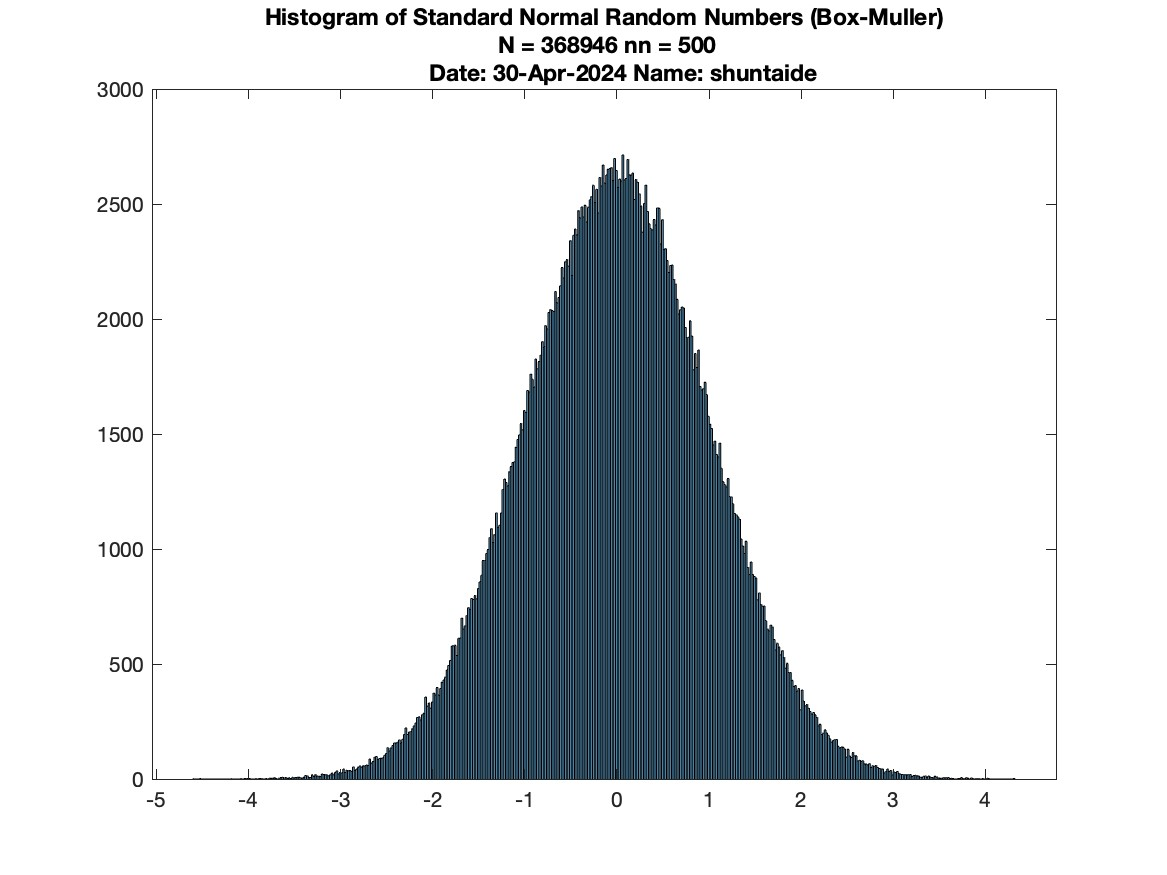
\includegraphics[width=0.8\textwidth]{src/figures/box-muller/Box-Muller_hist_N=368946_nn=500.jpg}
		\subcaption{ヒストグラム}
	\end{subfigure}
	\begin{subfigure}{0.48\linewidth}
		\centering
		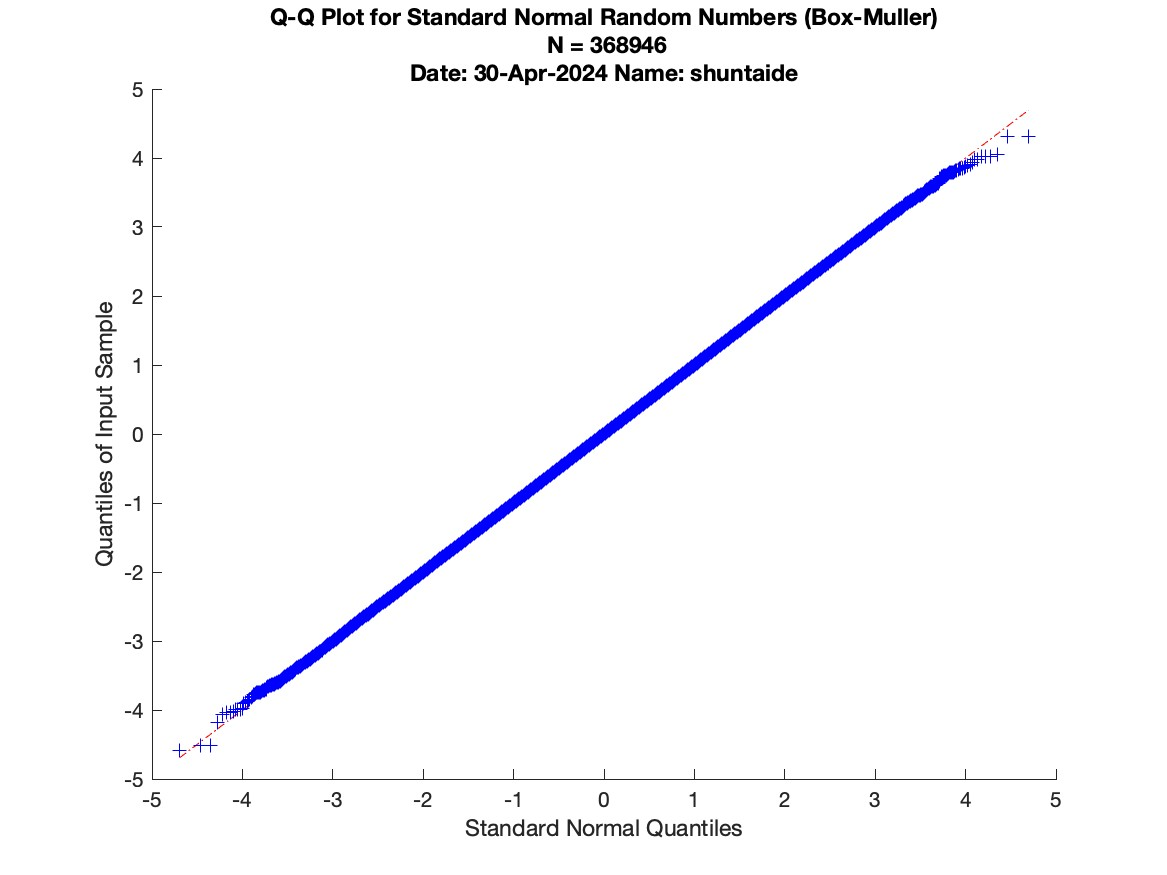
\includegraphics[width=0.8\textwidth]{src/figures/box-muller/Box-Muller_qqpl_N=368946.jpg}
		\subcaption{QQプロット}
	\end{subfigure}
	\caption{Box-Muller法による標準正規乱数の生成結果}\label{fig:box-muller-random}
\end{figure}
